\subsection{Model implementation (Jens Carl)}
The application model consists of the classes shown in figure \ref{fig:MVC_CD}. When a customer or admin logs into the application, a corresponding \texttt{User} sub-class object is instantiated. From the database, the logged-in user's credentials are found and put into the object. This object is then set in focus as the user currently logged in, e.g. \texttt{customerLoggedIn}. Controllers modify and use methods from this object when the user performs actions in the application. After an action is complete, the fields in the object are stored in the same table row as where it was fetched from, for future use. In figure \ref{fig:dbTables} below, the structure of the database is illustrated and described. 

\begin{figure}[H]
    \centering
    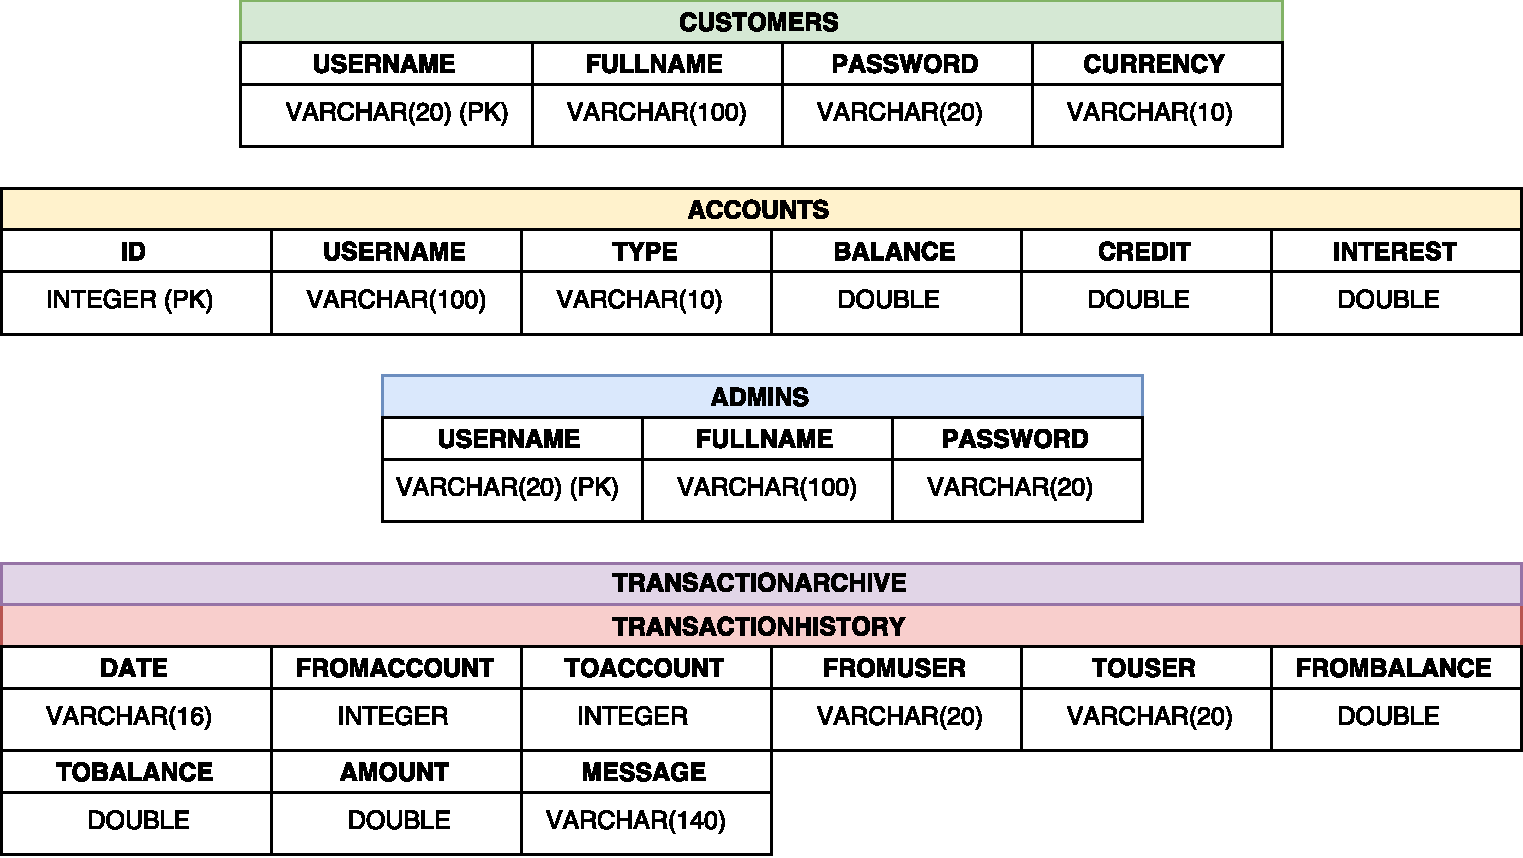
\includegraphics[width = 1.0\textwidth]{figures/dbTables.pdf}
    \caption{The table structure of the database was implemented to synergize with the operation procedure of the application. This means that, for example, the \texttt{ACCOUNTS}-table has roughly the same columns as fields in the \texttt{Account} java class. Likewise, this is true for tables \texttt{ADMINS} and \texttt{CUSTOMERS}, thus providing efficient and easy storage/fetching of required object constructor arguments for the application. 
    As the information required to store a transaction was spread across multiple Java objects, the table \texttt{TRANSACTIONHISTORY} was implemented otherwise. First we took a look at which elements we would like to store with a transaction, and then made a column for each of those. Later, a wrapper class \texttt{TransactionHistoryElement} was written in Java with fields equal to these columns. Table \texttt{TRANSACTIONARCHIVE} was created as a destination for migrating old transactions when performing batch jobs. It therefore has the same columns as \texttt{TRANSACTIONHISTORY}. Sample images of the database tables viewed in Data Studio can be seen in appendix section \ref{sec:apendixTables}.}
    \label{fig:dbTables}
\end{figure}



\subsubsection{Transaction History tables}
For a while we implemented dynamically generated tables. Each user had his/hers own table containing transaction history for that specific user. Later, however, this part of the model was replaced with just a single \texttt{TRANSACTIONHISTORY}-table holding all transactions in the bank. While dynamically generating tables seemed to provide an intuitive overview of data, we found it had two major flaws which proved to a deal-breaker: 1) it slowed down various operations substantially 2) it provided a sense of uncertainty about the current structure of the database, since the specific number of tables at any given time couldn't be predicted with certainty. 
%tables: customer, admin, accounts \\
%possible alternatives (dynamic, many tables) \\
%SQL statements, auto commit
             